

\section{A device taxonomy}
\labelsec{devbridge}

\href{https://137.204.107.21/syskb/it.unibo.iss2015intro/docs/Appls/ButtonLed/devBridge.html}{model of the Devices}
\href{https://137.204.107.21/syskb/it.unibo.iss2015intro/docs/Appls/ButtonLed/DevButtonBridge.jpg}{model of the Button}


\begin{center}
\begin{tabular}{ c }
     \includegraphics[scale = 0.45]{../../../it.unibo.iss2015intro/docs/Appls/ButtonLed/DevButtonBridge.jpg}\\
\end{tabular}{   }
\end{center}







\section{Problem Analysis}

\begin{itemize}
\item Define a (first) logic architecture
\end{itemize}

\lstinputlisting[language=java,caption={ \texttt{blsAnalysis2016.qa} }, firstline=1 ]{../../../it.unibo.bls2016.qa/src/blsAnalysis2016.qa}

 
\lstinputlisting[language=java,caption={ \texttt{blsAnalysisMsg.qa} }, firstline=1 ]{../../../it.unibo.bls2016.qa/src/blsAnalysisMsg.qa}

\newpage 
\section{From logical to physical
}
\subsection{Build and use a physical \textit{Button}}
\labelssec{exbutton}
Suppose that we have to solve to following problem:

\medskip 
\scriptsize
\framebox[15cm]{ %
\begin{minipage}{140mm}
Build a system that allows to a physical \textit{Button} connected to an \texttt{Arduino} device to emit a local event:\\ \texttt{\textbf{local\_click : clicked}} o
r a global event: \texttt{\textbf{click : clicked}}.
\end{minipage}}
\normalsize
\medskip    

In this example, the requirement or problem analysis phases probably end with the idea of a domain object able to interact with \texttt{Arduino} via the serial line. Conceptually, this object behaves as an \textit{observer} (in the \texttt{GOF} \textit{observer pattern} sense) of the serial port connected to \texttt{Arduino} and must be able to convert the observed input from the port into \texttt{qa} \textit{events}.
All this work can be defined by a proper conventional \java{} class.

\subsubsection{The code on \texttt{Arduino}.}
The code leaded into  \texttt{Arduino} is available in 

\begin{Verbatim}[fontsize=\scriptsize, frame=single , label=Arduino code site]
https://137.204.107.21/syskb/it.unibo.buttonLedSystem.arduino/arduino/blsMain/blsMain.ino
https://137.204.107.21/syskb/it.unibo.buttonLedSystem.arduino/arduino/blsMain/bls.h
https://137.204.107.21/syskb/it.unibo.buttonLedSystem.arduino/arduino/blsMain/bls.cpp
\end{Verbatim}

The \texttt{Arduino} writes on the Serial port strings formatted as \qa{} messages (see \xss{defmessages}):

%%\begin{Verbatim}[fontsize=\scriptsize, frame=single , label=Arduino output]
\begin{lstlisting}
msg( command, dispatch, arduinoLed13, connectedpc, ld13(V),0) 	with V=0 | 1  
\end{lstlisting}
%%\end{Verbatim}




 
\subsubsection{A \qa{} model of the system.}
Starting from this base, the application designer can define a \textit{project model} in which the details of the creation of a \texttt{DeviceButtonArduinoQa} object are delegated to a \prolog{} rule (\textit{createPojoButton}):

\lstinputlisting[language=ddr,caption={ \texttt{button2016.qa} }, firstline=1 , lastline=24 ]{../../src/button2016.qa}  

The \textit{createPojoButton} creation rule can be defined in the \texttt{buttonTheory} as follows :

\lstinputlisting[language=java,caption={ \texttt{buttonTheory.pl} }, firstline=1 ]{../../buttonTheory.pl}

\subsubsection{Referencing the current robot(actor).}
\labelssec{actorobj}
The \texttt{createPojoButton/4} rule binds (by using the predefined rule \texttt{actorobj/1} ) the variable \texttt{Actor} to a reference to the \java{} object that implements the actor \texttt{buttonobserver}. In this way the application designer can access in \prolog{} to all the public methods of the actor.  In our specific case, the rule gets the actor's standard output device (\texttt{OutView}) and then delegates the creation of the button  to a static method of the  \java{} class \texttt{DeviceButtonArduinoQa}


\subsubsection{An event observer.}
To facilitate the testing of the system so far defined, the application designer could introduce an actor \texttt{buttonobserver} with the task to perceive the events emitted by the \texttt{button} and to simulate the control of a \textit{led}.  

\lstinputlisting[language=ddr,caption={ \texttt{button2016.qa} }, firstline=25  ]{../../src/button2016.qa}  

The sentences:

\begin{Verbatim}[fontsize=\scriptsize, frame=single]
/* (1) */ sense time(600000) local_click ->  continue ;
/* (2) */ [ !?ledSwitch(V) ] onEvent local_click : ANY -> println( buttonobserver(led(V)) ) ;
\end{Verbatim}

specify the following behaviour:

\medskip 
\scriptsize
\framebox[15cm]{ %
\begin{minipage}{140mm}
\texttt{(1)} Wait for the event local\_click. \texttt{(2)}\\
When the event occurs, check the guard \texttt{ledSwitch(V)} and (wit no reference to any particular event content) write the current state of the led given by the variable \texttt{V}.
\end{minipage}}
\normalsize
\medskip

The \texttt{buttonobserverTheory} loaded in the \texttt{init} plan by the actor \texttt{buttonobserver} defines the rule for \texttt{ledSwitch(V)}:

\lstinputlisting[language=java,caption={ \texttt{buttonobserverTheory.pl} }, firstline=1 ]{../../buttonobserverTheory.pl}

\subsection{Build a virtual \textit{Led} able to react to events}
\labelssec{exled}
Suppose that we have to solve to following problem:

\medskip 
\scriptsize
\framebox[15cm]{ %
\begin{minipage}{140mm}
Build a system that provides an actor able to react to events of the form:\\
\texttt{\textbf{local\_click : clicked}} or: \texttt{\textbf{click : clicked}}\\
by modifying the state of a virtual Led implemented by a conventional GUI.
\end{minipage}}
\normalsize
\medskip    


In this example, the requirement or problem analysis phases probably end with the idea of a domain entity able to perceive \textit{events}, conceptually working as an \textit{observer} in an \textit{event-driven} or \textit{event-based} sense (see \xss{defevents}). Such an entity can be modelled as a \qa{} able to reacts to \textit{events} by changing the state of a conventional GUI by means of a proper conventional \java{} class, like the following one: 

\lstinputlisting[language=java,caption={ \texttt{DeviceDeviceLedGui.java} }, firstline=1 ]{../../src/it/unibo/devices/qa/DeviceLedGui.java}

\subsubsection{A \qa{} model of the system.}
The application designer can now define the following  \textit{project model}  :

\lstinputlisting[language=ddr,caption={ \texttt{buttonLed2016.qa} }, firstline=1 , lastline=29 ]{../../src/buttonLed2016.qa}  

The \textit{createLed/2} creation rule can be defined in the \texttt{ledTheory} as follows :

\lstinputlisting[language=java,caption={ \texttt{ledTheory.pl} }, firstline=1 , lastline=15 ]{../../ledTheory.pl} 

To facilitate the testing, the application designer could complete the system with the actor \texttt{button} introduced in \xss{exbutton}.  

\lstinputlisting[language=ddr,caption={ \texttt{buttonLed2016.qa} }, firstline=30  ]{../../src/buttonLed2016.qa}  

\subsection{Work todo.}
The led example should be completed by the reader with the introduction of a proper \texttt{ledSwitch} rule in the \texttt{ledTheory}.
The reader is invited to submit the proposed solution to the author of this notes before the 9 of March 2016.

The next step could be the introduction of a physical \textit{Led} or a physical \textit{Button} connected to a \textit{Raspberry} device. The \textit{Raspberry} could be directly connected to \textit{Arduino} or to a conventional computer. Another step could be the implementation of the \textit{Button} on an \textit{Android} device. 

\section{From the button-led system to \texttt{IOT} application.}
More generally, a Button-Led system (\texttt{BLS}) could have an open-ended set of local or distributed configurations:

\begin{center}
\begin{tabular}{ c }
     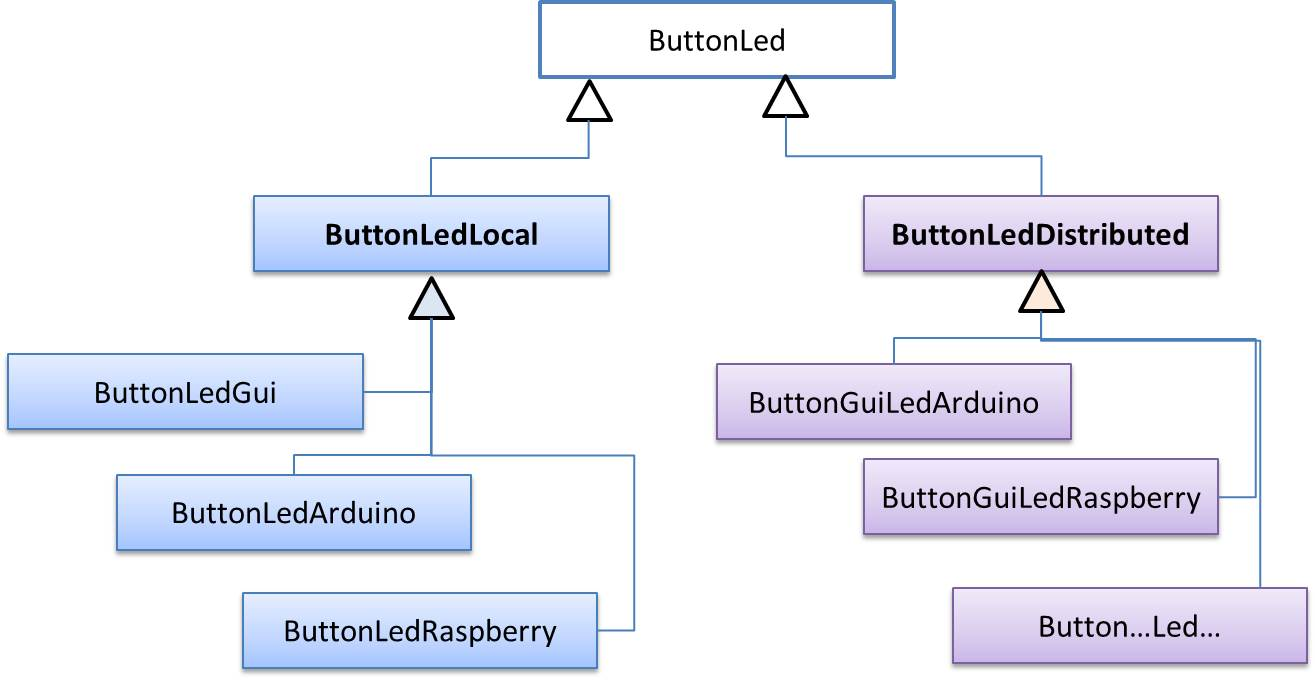
\includegraphics[scale = 0.45]{img/blsall.jpg}\\
\end{tabular}{   }
\end{center}

The problem is how to conceive a software organization that allows our software company to face all the possible configurations by limiting as much as possible code re-factoring. The \textit{vision} here is to build a software architecture easily adaptable to each different, specific (technological) configuration. 

Thus, a work to do is to compare the actor model-driven approach followed in this paper with a traditional object-oriented / pattern-based approach.

In this perspective the \texttt{BLS} can be viewed as a point in the space of the \texttt{IOT} applications that allows us to discuss many typical problems in this field. For example, we can discuss how the \texttt{BLS} system could be designed and developed by following a traditional oo-design. A possible evolution of oo-models for the logical architecture of the system can be summarized by following picture:


\begin{center}
\begin{tabular}{ c }
     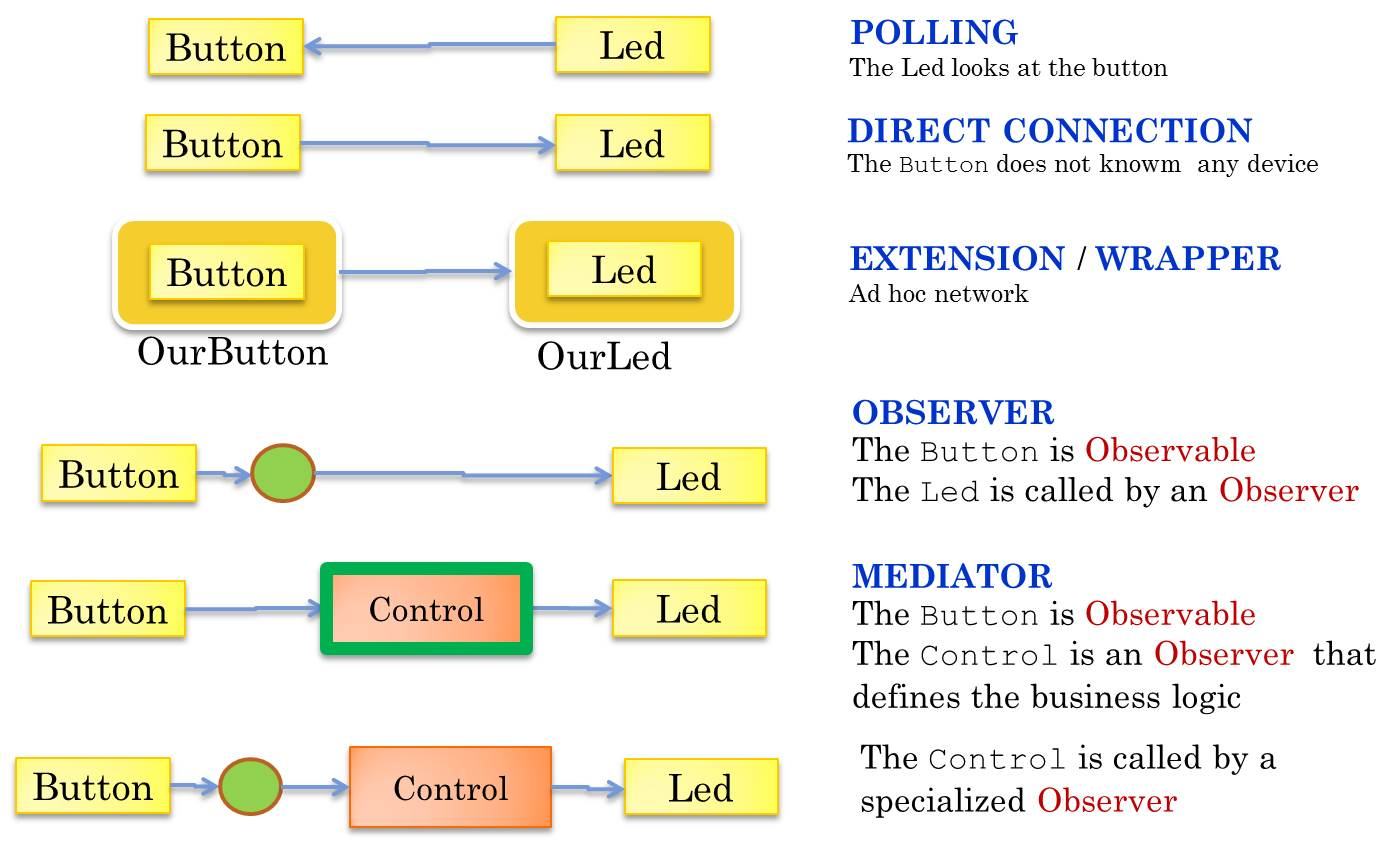
\includegraphics[scale = 0.45]{img/blsInteraction0.jpg}\\
\end{tabular}{   }
\end{center}

A further evolution could be related to the introduction of the pattern bridge:

\begin{center}
\begin{tabular}{ c }
     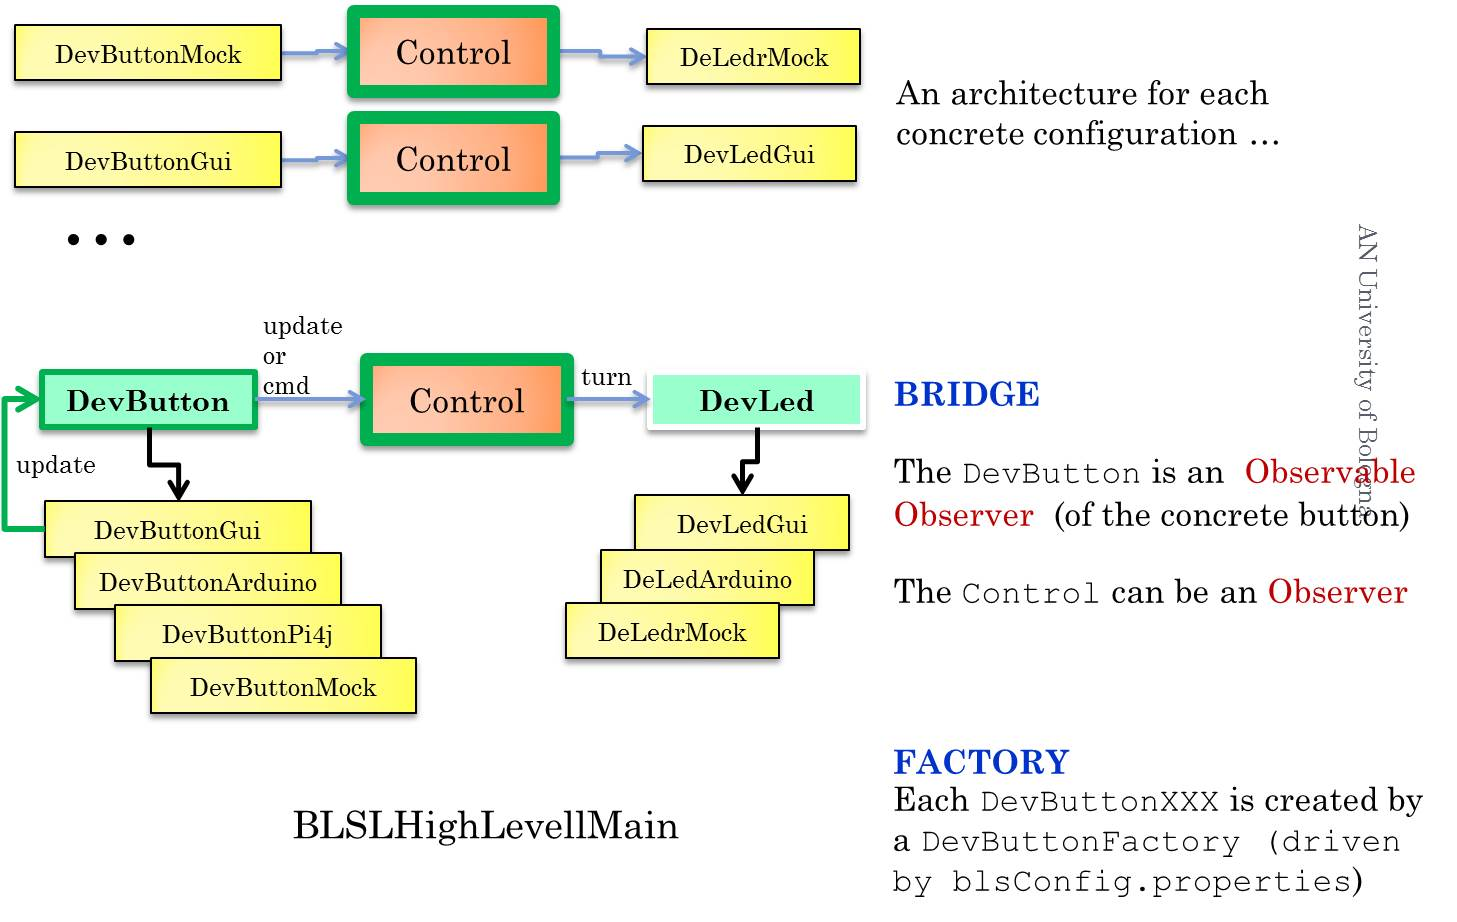
\includegraphics[scale = 0.45]{img/blsInteraction1.jpg}\\
\end{tabular}{   }
\end{center}


This kind of 'traditional' object oriented approach in the design and development of a \texttt{BLS} is described in docs/Appls/ButtonLed/logicArch.html. It has lead to the development of two main libraries:

\begin{itemize}
\item \texttt{blsHL.jar} from project  \textit{it.unibo.buttonLedSystemHL} : 
\item \texttt{blsGUI.jar} from project \textit{it.unibo.buttonLedSystem.gui} : 
\end{itemize}

These libraries can be help in reducing the cost of software development also in the case of distributed heterogeneous systems, if we are able to design (model) and build the systems with entities able to work according to message.passing or event-based paradigms while being at the same time able to reuse traditional software. The techniques presented in this work demonstrate that this vision is possible.

%%showing how 'traditional'  oo software can be reused in actor-based, model-driven software development by exploiting the techniques presented in this work.. 
